\newpage
	\subsection{Component Diagrams}
        \subsubsection{Request For Printing Service}
        \begin{center}
        \begin{figure}[!htp]
        \begin{center}
         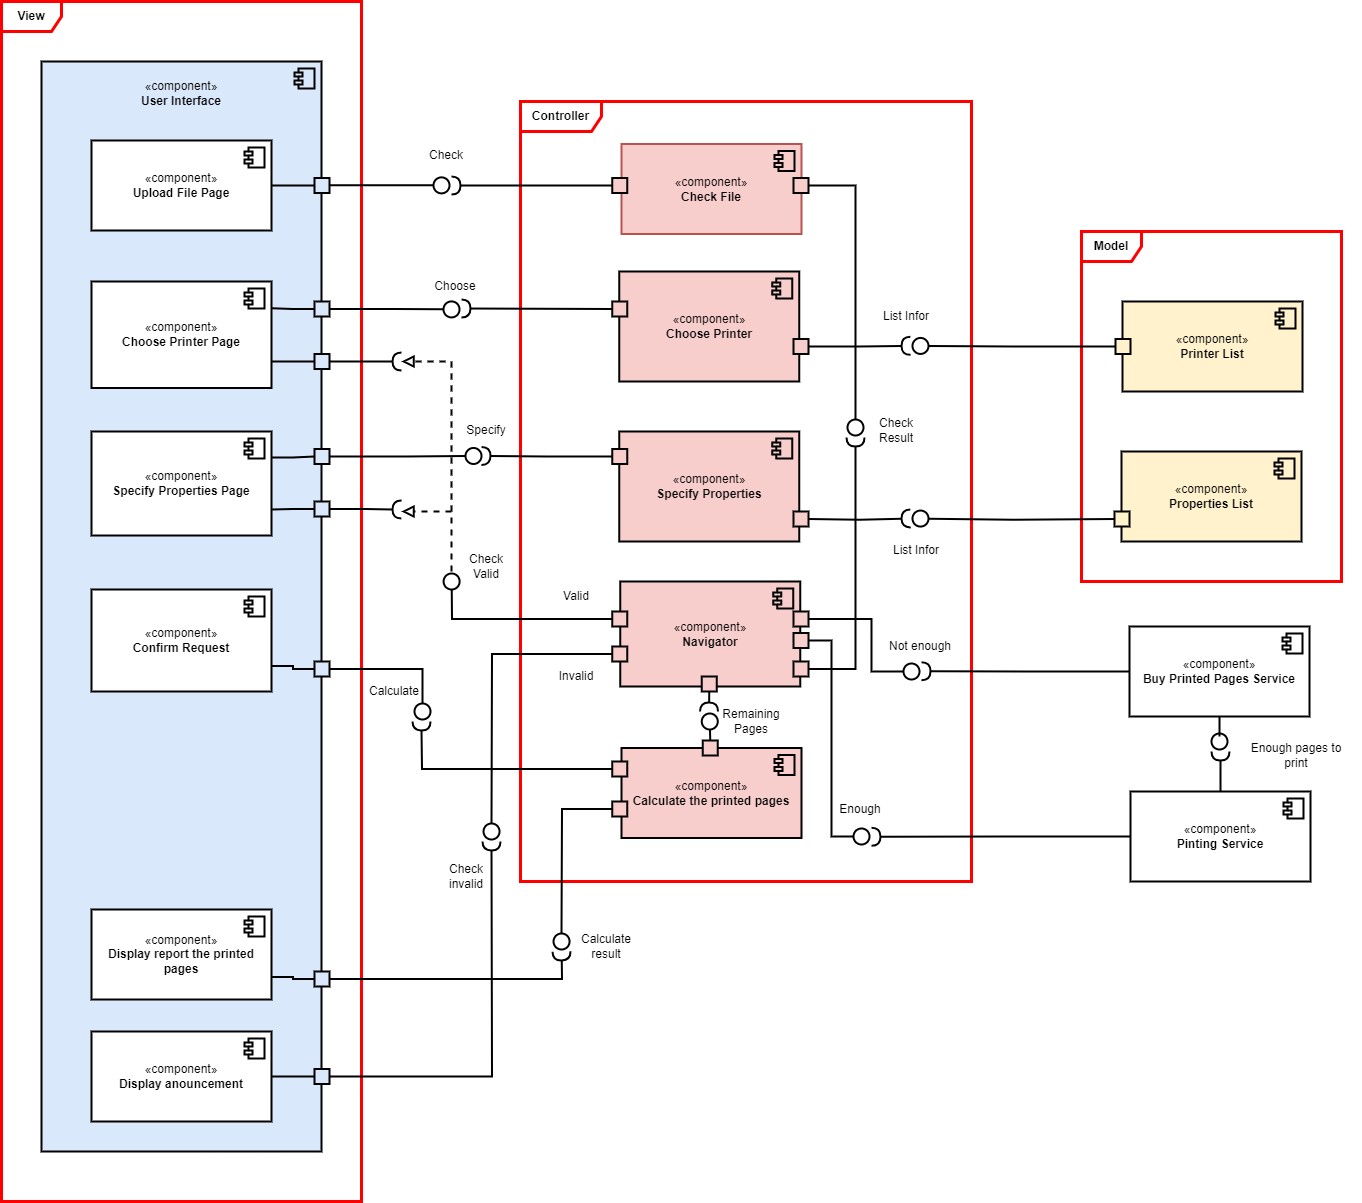
\includegraphics[scale=0.31]{images/Task3/Component Diagrams/RequestForPrintingService.png}
        \end{center}
        \end{figure}
        \end{center}

        \newpage
        \textbf{Mô tả:}
        \begin{itemize}
            \item File khi được tải lên hệ thống sẽ được khối \textit{Check File} kiểm tra và gửi thông tin đến khối \textit{Navigator} để phân chia luồng xử lý:
            \begin{itemize}
                \item Nếu file không hợp lệ, \textit{Display anouncement} sẽ thông báo đến người dùng.
                \item Nếu file hợp lệ \textit{Choose Printer Page} và \textit{Specify Properties Page} sẽ được kích hoạt cho phép người dùng sử dụng.
            \end{itemize}
            \item \textit{Choose Printer Page} và \textit{Specify Properties Page} khi được kích hoạt bởi người dùng sẽ được xử lý lần lượt bởi các khối \textit{Choose Printer} và \textit{Specify Propertries}. Hai khối trên dựa vào yêu cầu của người dùng và thông tin trong \textit{Printer List}, \textit{Properties List} để xử lý.
            \item Sau khi hoàn tất các thao tác trên người dùng sẽ phải xác nhận yêu cầu \textit{Confirm Request} để tiếp tục, khối \textit{Calculate the printed pages} sẽ tính toán và gửi báo cáo đến người dùng xem họ còn lại bao nhiêu trang có thể in đồng thởi gửi tín hiệu đến khối \textit{Navigator}:
            \begin{itemize}
                \item Nếu số trang còn lại đủ để in tài liệu, \textit{Printing Service} sẽ kết nối với máy in và tiến hành in hoàn tất quá trình.
                \item Nếu số trang không đủ người dùng được chuyển đến chức năng \textit{Buy Printed Pages Service} để mua thêm trang in. Sau khi mua đủ số trang in cần thiết người dùng sẽ được chuyển đến \textit{Printing Service}để hoàn tất.
            \end{itemize}
        \end{itemize}

        \newpage
        \subsubsection{Make Online Payment}
        \begin{center}
        \begin{figure}[!htp]
        \begin{center}
         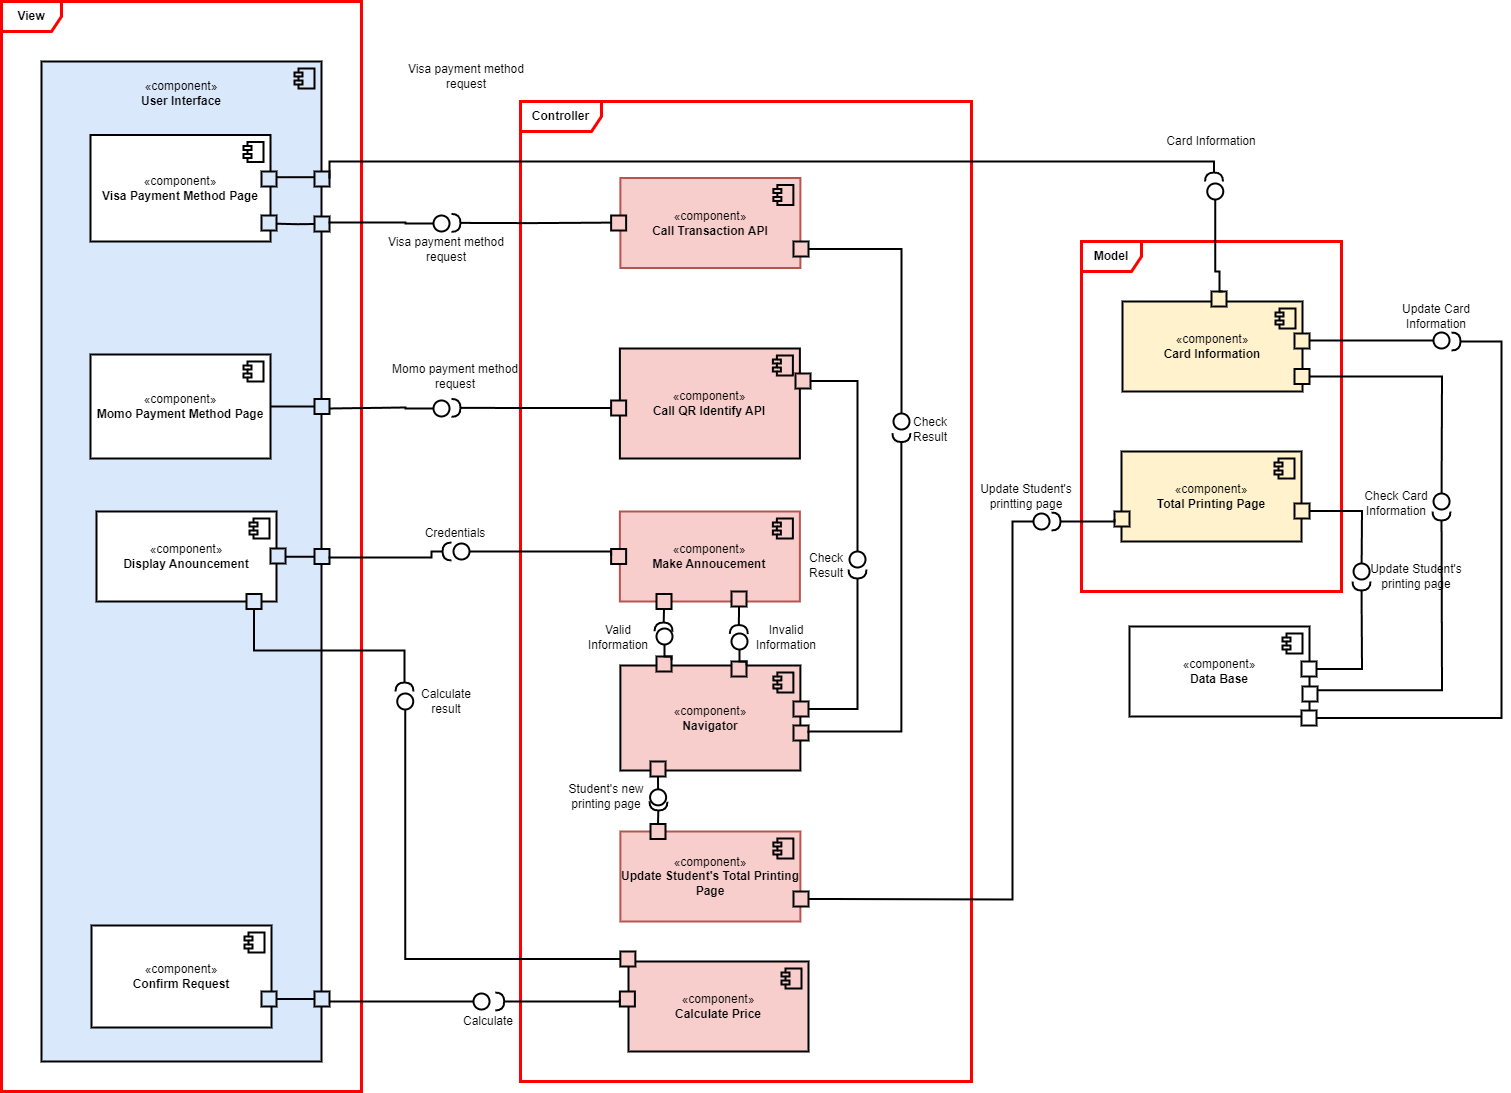
\includegraphics[scale=0.32]{images/Task3/Component Diagrams/paymentComponentDiagram.drawio.png}
        \end{center}
        \end{figure}
        \end{center}
        \newpage
        \textbf{Mô tả:}
        \begin{itemize}
            \item Tại giao diện \textit{Confirm Request} khi người dùng chọn số lượng trang in và đồng ý thì khối \textit{Calculate Price} sẽ thực hiện tính toán giá tiền và hiển thị cho người dùng thông qua khối \textit{Display Anouncement}. Đồng thời cũng tại giao diện này người dùng sẽ chọn phương thức thanh toán.
            \item Tại giao diện \textit{Visa Payment Method}, nếu thông tin về visacard của người dùng được đối chiếu qua khối \textit{Card Information} và \textit{Data Base} là hợp lệ thì thông tin thẻ sẽ được khối \textit{Call Transaction API} xử lí và thực hiện thanh toán. Còn nếu thông tin về thẻ không tồn tại thì người dùng sẽ nhập thông tin về thẻ trong giao diện \textit{Visa Payment Method} và khối \textit{Card Information} sẽ gửi yêu cầu Update Card Information đến khối \textit{Data Base}. Sau đó thông tin sẽ được khối \textit{Call Transaction API} xử lí và thực hiện thanh toán.
            \item Tại giao diện \textit{Momo Payment Method}, người dùng sẽ quét mã QR và thông tin này sẽ được khối \textit{Call QR Identify API} xử lí và thực hiện thanh toán.
            \begin{itemize}
                \item Trường hợp thông tin thanh toán chính xác: khối \textit{Navigator} sẽ tiến hành gửi số lượng trang in mới của sinh viên đến khối \textit{Update Student's Total Printting Page } và khối này sẽ gửi yêu cầu đến khối \textit{Total Printting Page} trong Model và cập nhật thông tin trong database.
                \item Trường hợp thông tin xác thực không chính xác: Người dùng có thể tiến hành nhập lại thông tin về thẻ thông qua giao diện \textit{Visa Payment Method} (trong trường hợp thanh toán qua visacard), quét lại mã QR qua giao diện \textit{Momo Payment Method} (trong trường hợp thanh toán qua momo) hoặc thoát khỏi qua trình mua trang in.    
            \end{itemize}
        \end{itemize}


        \newpage
        \subsubsection{Manage Printers}
        \begin{center}
        \begin{figure}[!htp]
        \begin{center}
         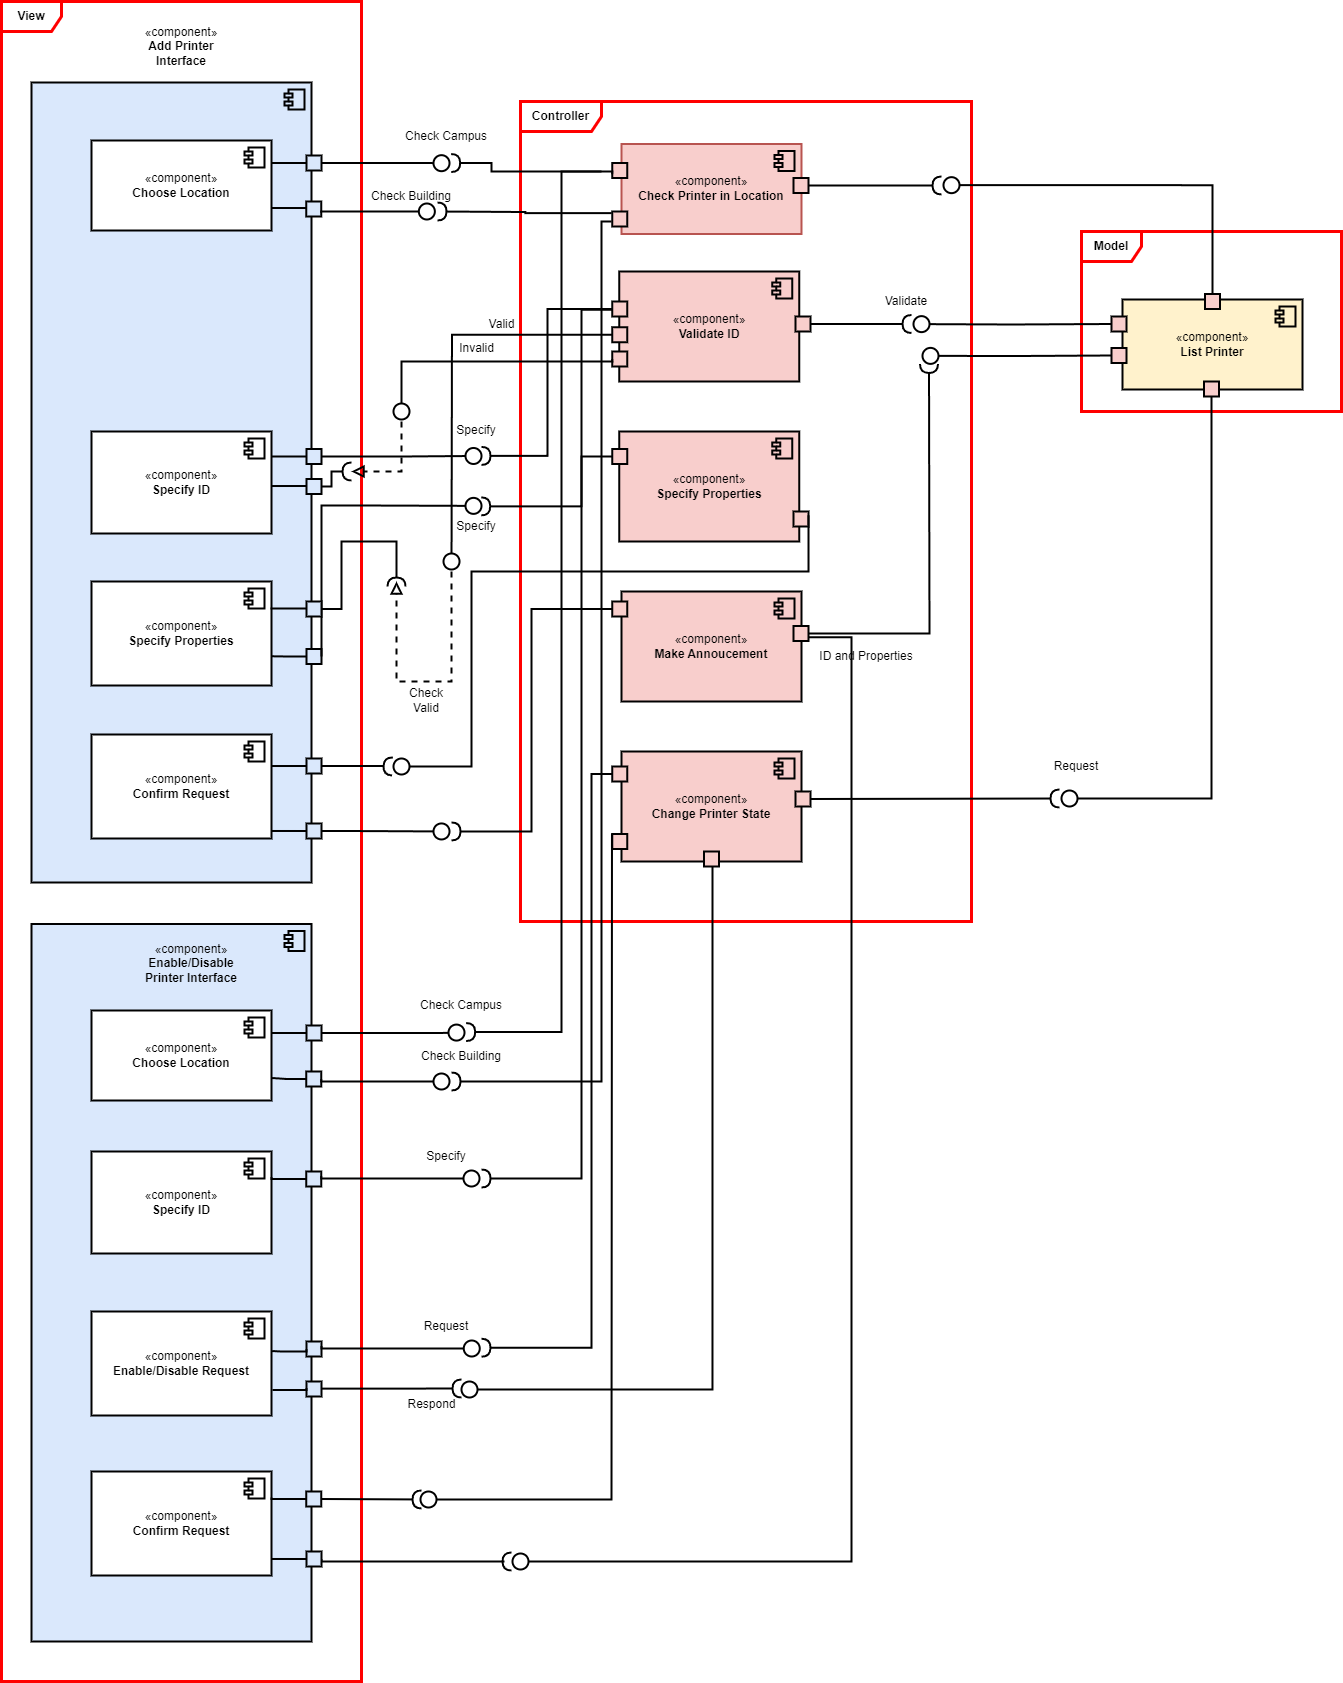
\includegraphics[scale=0.31]{images/Task3/Component Diagrams/ManagePrinterComponentDiagram.png}
        \end{center}
        \end{figure}
        \end{center}

        \newpage
        \textbf{Mô tả:}
        \begin{itemize}
            \item Tại giao diện \textit{Add Printers}, SPSO sẽ chọn cơ sở (campus) và tòa nhà (building) có sẵn, sau đó sẽ nhập ID của máy in mới muốn thêm vào hệ thống. ID đó sẽ đi qua khối \textit{Validate ID} để kiểm tra, nếu hợp lệ sẽ hiển thị hợp lệ và SPSO sẽ tiếp tục nhập các thông tin khác của máy in. Nếu không hợp lệ, tín hiệu sẽ được gửi đến khối \textit{Make Annoucement}, khối trả về thông báo ID không hợp lệ và SPSO sẽ phải nhập lại. Sau khi đã hoàn tất nhập các thông tin, SPSO sẽ nhấn Xác nhận và lưu thông tin vào Hệ thống các máy in.
            \item Tại giao diện \textit{Enable/Disable Printer}, SPSO sẽ chọn cơ sở (campus) và tòa nhà (building) có sẵn, sau đó sẽ nhập ID của máy in muốn thay đổi trạng thái. Nếu ID hợp lệ, khối \textit{Make Annoucement} trả về thông báo hợp lệ, SPSO có thể thay đổi trạng thái của máy in như mong muốn. Nếu không hợp lệ, tín hiệu sẽ được gửi đến khối \textit{Make Annoucement}, khối trả về thông báo ID không hợp lệ và SPSO sẽ phải nhập lại. Sau khi đã xác nhận trạng thái, SPSO có thể xác nhận thay đổi và khối \textit{Change Printer State} sẽ thay đổi trạng thái của máy in.
        \end{itemize}



        \newpage
        \subsubsection{Configure System}
        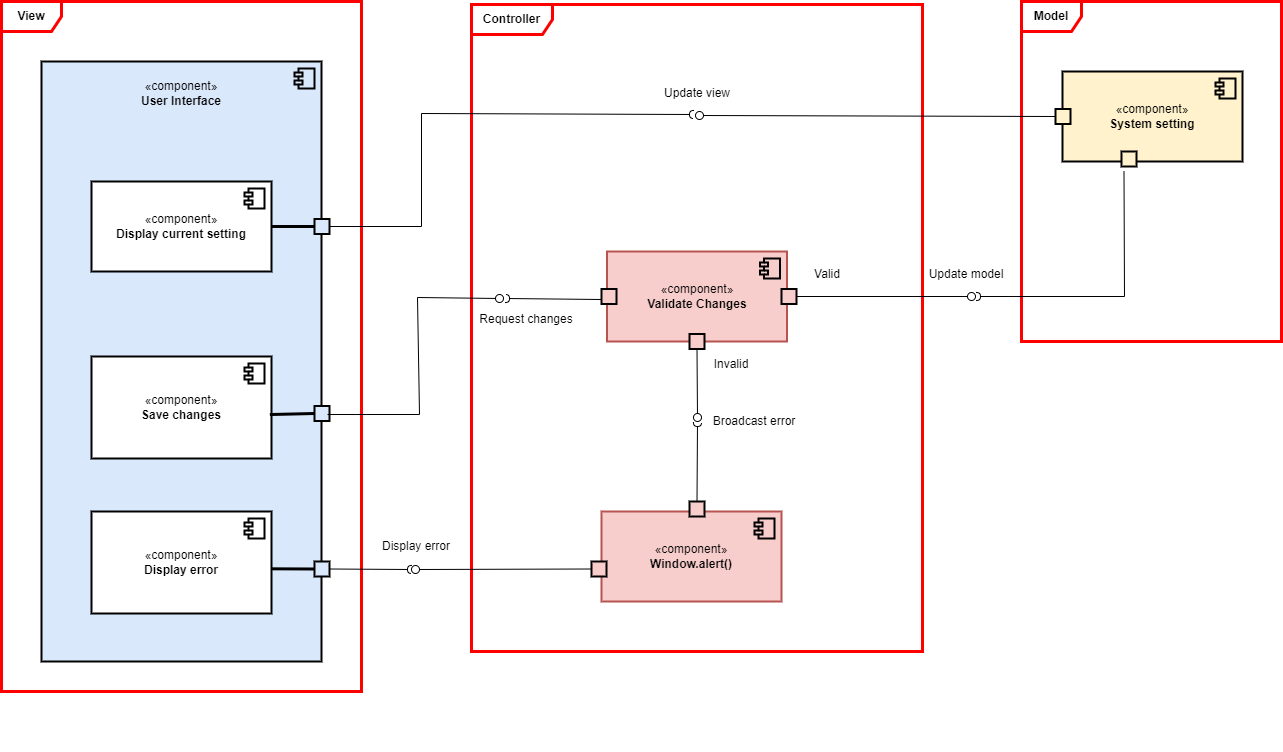
\includegraphics[width=\textwidth]{images/Task3/Component Diagrams/ConfigureSystemComponentDiagram.drawio.png}
        \textbf{Mô tả:}
        Thao tác thay đổi các thiết lập của hệ thống bao gồm các component chính là Display current setting ở phần view, Validate changes ở phần Controller và System setting ở phần model.
        \begin{itemize}
            \item Khi vào trang thay đổi các thiết lập của hệ thống, System setting sẽ cập nhật các thông tin hiển thị cho người dùng bằng dữ liệu được lưu trong hệ thống.
            \item Nếu người dùng lưu thay đổi, Controller sẽ tiếp nhận việc kiểm tra dữ liệu được thay đổi.
            \item Nếu dữ liệu mới hợp lệ, controller sẽ tiến hành giao tiếp với model để cập nhật system setting và system setting sẽ cập nhật lại giao diện người dùng bằng dữ liệu mới.
            \item Nếu dữ liệu mới không hợp lệ, controller gọi hàm window.alert để báo lỗi lên giao diện người dùng.
        \end{itemize}

        \newpage
	\subsubsection{Log In}
        \begin{center}
        \begin{figure}[!htp]
        \begin{center}
         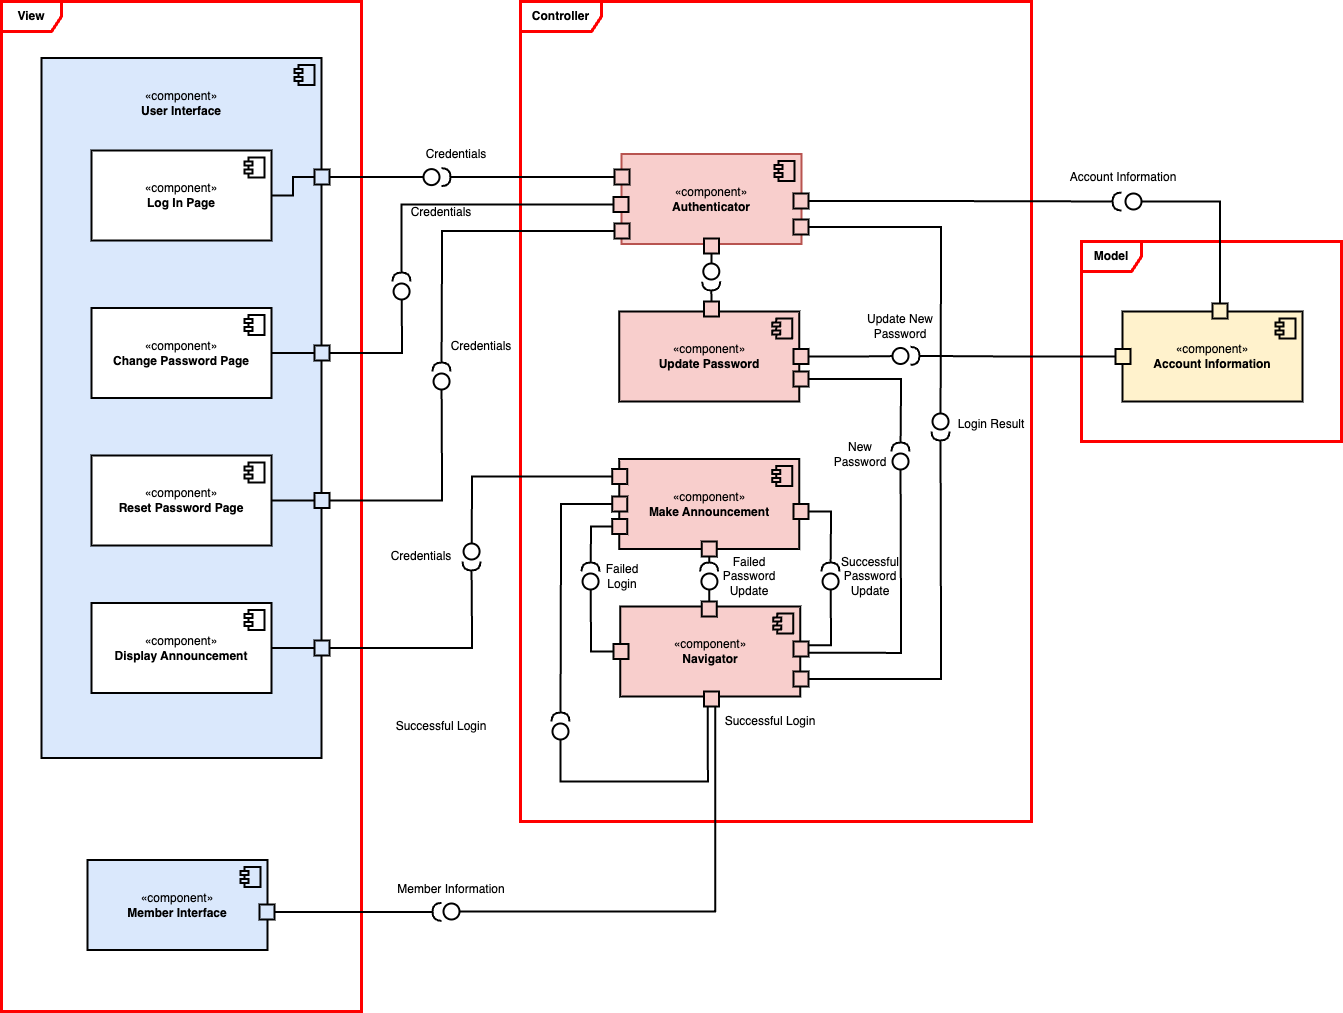
\includegraphics[scale=0.31]{images/Task3/Component Diagrams/ComponentDiagramLogin.drawio.png}
        \end{center}
        \end{figure}
        \end{center}

        \newpage
	\textbf{Mô tả:}
        \begin{itemize}
            \item Tại giao diện đăng nhập \textit{(Login Page)}, người dùng cung cấp các thông tin xác thực theo yêu cầu \textit{(username, password)}. Thông tin này sẽ được khối \textit{Authenticator} tiếp nhận và đối chiếu với dữ liệu từ \textit{Account Information} trong model. Sau đó kết quả được gửi đến khối \textit{Navigator} để tiến hành điều hướng, đồng thời thông báo đến cho người dùng qua khối \textit{Display Announcement}.
            \begin{itemize}
                \item Trường hợp thông tin đăng nhập chính xác: Người dùng sẽ được điều hướng đến giao
                diện dành cho thành viên với các thông tin của tài khoản đó..
                \item Trường hợp thông tin xác thực không chính xác: Người dùng có thể tiến hành đăng nhập lại hoặc chọn đặt lại mật khẩu (\textit{Reset password}).    
            \end{itemize}
            \item Tương tự, tại giao diện thay đổi mật khẩu (\textit{Change Password}) và đặt lại mật khẩu (\textit{Reset Password}), người dùng cũng cần nhập các thông tin xác thực cần thiết (\textit{username, old password, new password, confirm password} đối với \textit{Change Password} và \textit{username, email, new password, confirm password} đối với \textit{Reset Password}). Khối \textit{Authenticator} sẽ tiếp nhận và tiến hành xác thực các thông tin này với dữ liệu từ \textit{Account Information}. Kết quả xác thực này sẽ được gửi đến khối \textit{Navigator} để tiến hành điều hướng thích hợp và thông báo đến người dùng qua khối \textit{Display Announcement}.
            \begin{itemize}
                \item Trường hợp thông tin đăng nhập chính xác: Khối \textit{Update Password} sẽ được kích hoặc và tiến hành cập nhật lại mật khẩu mới vào tài khoản người dùng.
                \item Trường hợp thông tin xác thực không chính xác: Người dùng cần tiến hành nhập thông tin xác thực lại.
            \end{itemize}
        \end{itemize}